\documentclass{article}

\usepackage[english]{babel}
\usepackage{amsmath}
\usepackage{amssymb}
\usepackage{amsthm}
\usepackage[font=small]{caption}
\usepackage{cite}
\usepackage{graphicx}

\newtheorem{algorithm}{Algorithm}
\newtheorem{definition}{Definition}
\newtheorem{example}{Example}
\newtheorem{lemma}{Lemma}
\newtheorem{proposition}{Proposition}
\newtheorem{remark}{Remark}

%---------------------------------------------------------------

\title{Analytic combinatorics for bioinformatics I: applications to
seeding methods}
%\author{
%\textsc{Guillaume Filion} \\ [1ex]
%\normalsize CRG, Barcelona
%}
\date{\today}

%---------------------------------------------------------------
%---------------------------------------------------------------


\begin{document}

\maketitle

\begin{abstract}
Text of the abstract.
\end{abstract}


%---------------------------------------------------------------
%---------------------------------------------------------------

\section{Introduction}

Computing the best alignment between two sequences is carried out by
dynamic programming. However, the running time of these algorithms scale
$O(mn)$, where $m$ and $n$ are the sequence lengths, so it is only
feasible for short sequences. For long sequences, heuristics are used for
speed up, and the most popular belong to ``seeding'' methods.

This document is predominantly written for bioinformaticians and people
with a working knowledge of sequencing technologies and their applications.
Accordingly, the focus will be on explaining the mathematical concepts,
rather than the technological aspects. Also, our goal here is not to push
the boundaries of analytic combinatorics, but to explain how its simplest
concepts are useful to solve common problems in bioinformatics. We have
opted for simplicity, to the detriment of generality and rigor. The
results presented here are only a basic introduction to analytic
combinatorics; the field is currently much more advanced and we refer the
interested to the original literature.

\section{Weighted generating functions}
\label{sec:WGF}

\begin{definition}
\label{def:GF}
Let $\mathcal{A}$ be a set of combinatorial objects characterized by a
size and a weight. The weighted generating function of $\mathcal{A}$ is
defined as

\begin{equation}
\label{eq:GF1}
A(z) = \sum_{a \in A} w(a) z^{|a|},
\end{equation}

\noindent
where $|a|$ and $w(a)$ denote the size and weight of an object $a$,
respectively. This also defines a sequence $(a_k)_{k \geq 0}$ such that 

\begin{equation}
\label{eq:GF2}
A(z) = \sum_{k=0}^\infty a_k z^k.
\end{equation}

By definition $a_k = \sum_{a \in A_k}w(a)$, where $A_k$ is the class of
objects of size $k$. The number $a_k$ is called the total weight of
objects of size $k$.
\end{definition}

Note that in definition \ref{def:GF}, the weight is a property of
combinatorial objects and the total weight is a property of a classes of
ojects. Expressions (\ref{eq:GF1}) and (\ref{eq:GF2}) are equivalent.
Depending on the context, we will use one or the other.

The essence of analytic combinatorics is that some operations on
combinatorial objects correspond to some operations on their generatintg
function. If $A(z)$ and $B(Z)$ are the weighted generating functions of
two mutually exclusive sets $\mathcal{A}$ and $\mathcal{B}$, the weighted
generating function of $\mathcal{A} \cup \mathcal{B}$ is $A(z) + B(z)$, as
appears immediately from expression (\ref{eq:GF1}). Size and weight can be
extended to pairs of objects in $\mathcal{A} \times \mathcal{B}$ by
defining $|(a,b)| = |a| + |b|$ and $w(a,b) = w(a)w(b)$. With this
convention, the weighted generating function of $\mathcal{A} \times
\mathcal{B}$ is $A(z)B(z)$, as shown by expression (\ref{eq:GF1})
once again

\begin{equation*}
A(z)B(z) =
\sum_{a\in \mathcal{A}}w(a)z^{|a|} \sum_{b\in \mathcal{B}}w(b)z^{|b|}
= \sum_{(a,b) \in \mathcal{A} \times \mathcal{B}} w(a)w(b)z^{|a|+|b|}.
\end{equation*}

\begin{example}
\label{ex:simple}
Assume that $\mathcal{A}$ contains a single object $a$ of size $1$ and of
weight $p$. The weighted generating function of $\mathcal{A}$ is $pz$.
The set $\mathcal{A}^2$ contains a single object $(a,a)$ of size $2$ and
weight $p^2$. Its weighted generating function is $p^2z^2 = pz \cdot pz$.
\end{example}

The definition of size and weight can be further extended to any finite
Cartesian product in the same way. The generating function of a cartesian
product then comes as the product of their generating functions.

\begin{example}
\label{ex:sequences}
Following up on example~\ref{ex:simple}, the set $\mathcal{A}^k$ contains
a single object of size $k$ and weight $p^k$, and its weighted generating
function is $p^kz^k$. Since the sets $\mathcal{A}, \mathcal{A}^2,
\mathcal{A}^3,\ldots$ are mutually exclusive, the weighted generating
function of their union is

\begin{equation*}
pz + (pz)^2 + (pz)^3 \ldots
\end{equation*}

For any given $k$, notice that $(1-pz) \big(pz + (pz)^2 + \ldots + (pz)^k
\big) = pz-(pz)^{k+1}$.  If $|z| < 1/p$, the term $(pz)^{k+1}$ vanishes as
$k$ increases. So the weighted generating function is defined for $|z| <
1/p$ and is equal to

\begin{equation*}
pz + (pz)^2 + (pz)^3 \ldots = \frac{pz}{1-pz}.
\end{equation*}
\end{example}

Example~\ref{ex:sequences} can be generalized. For any set $\mathcal{A}$,
objects of $\mathcal{A}^+ = \cup_{k=1}^\infty\mathcal{A}^k$ are called
nonempty sequences of objects of $\mathcal{A}$. By defining
$\mathcal{A}^0$ as the set containg only $\varepsilon$, the ``empty''
object of size 0 and weight 1, we can also define $\mathcal{A}^* =
\cup_{k=0}^\infty\mathcal{A}^k$ as the set of sequences of objects of
$\mathcal{A}$.

\begin{proposition}
\label{th:sequences}
Let $\mathcal{A}$ be a set with weighted generating function $A(z)$. The
generating functions of $\mathcal{A}^+$ and $\mathcal{A}^*$ are defined
for $|A(z)| < 1$ and are respectively equal to

\begin{equation*}
\begin{split}
\frac{A(z)}{1-A(z)}&\text{, and} \\
\frac{1}{1-A(z)}&.
\end{split}
\end{equation*}
\end{proposition}

\begin{proof}
For $k \geq 1$, the generating function of $\mathcal{A}^k$ is $A(z)^k$ and
since the sets are mutually exclusive, the weighted generating function of
their union $\mathcal{A}^+$ is $A(z) + A(z)^2 + \ldots = A(z) / (1-A(z))$,
provided $|A(z)| < 1$.

The generating function of $\mathcal{A}^0$ is $1$ so the weighted
generating function of $\mathcal{A}^*$ is $1 + A(z) + A(z)^2 + \ldots =
1 / (1-A(z))$, provided $|A(z)| < 1$.
\end{proof}

\begin{remark}
These expressions are not defined for $A(z) = 1$, \textit{i.e.} when
$\mathcal{A}$ contains only the empty object. In other words, one cannot
construct sequences of empty ojects.
\end{remark}

From here on, we will not state the conditions of definition of the
generating functions. We will simply assume that $|z|$ is lower than the
radius of convergence of the given expression.

These simple rules are enough to solve non-trivial problems. We now
motivate the analytic combinatorics approach by a simple example that has
no direct connection with seeding algorithms, but that will nevertheless
be useful for exposition purposes.

\begin{example}
\label{ex:Sanger}
In Sanger sequencing, a nucleotide is sometimes duplicated because the
corresponding peak is wider than average. A nucleotide thus has size $1$
with a certain probability $q$, and size $2$ with probability $p = 1-q$.
The weighted generating function of nucleotides is thus $qz + pz^2$. Reads
are sequences of nucleotides, so by proposition~\ref{th:sequences} they
have weighted generating function

\begin{equation}
\label{eq:Sanger}
\frac{1}{1-qz-pz^2}.
\end{equation}
\end{example}

In this example, what is the probability that a read of size $100$ has no
duplication? The first answer coming to mind is $q^{100}$, but this is the
probability that a read of $100$ \emph{nucleotides} has no duplication. To
answer the question, we need to divide $q^{100}$ by the cumulated
probabilities of reads of size $100$. We can express this quantity from
the binomial distribution as

\begin{equation*}
{100 \choose 0}q^{100} + {99 \choose 1}pq^{99} + {98 \choose 2}p^2q^{98} +
\ldots + {50 \choose 50}p^{50}.
\end{equation*}

This is not straightforward to compute, but it happens to be the
coefficient of $z^{100}$ in the series expansion of (\ref{eq:Sanger}).
Indeed, from the definition expressed in formula (\ref{eq:GF1}), the
coefficient of $z^{100}$ is the sum of the weights of all objects of size
$100$.  Solving the problem is a matter of evaluating this coefficient.

%%%%%%%%%%%%% The crown jewel proposition %%%%%%%%%%%%%

It is not always possible to obtain exact values, but one of the crown
jewels of analytic combinatorics is that we can very accurately
approximate the coefficients of weighted generating functions.  In order
to show how to do this, we will first prove a more general result.

\begin{proposition}
\label{th:ass}
If a weighted generating function $A(z)$ is the ratio of two polynomials
$P(z)/Q(z)$, and that the roots of $Q$ are simple, then the coefficient of
$z^k$ in its series expansion is asymptotically equivalent to

\begin{equation}
\label{eq:ass}
-\frac{P(z_1)}{Q'(z_1)}\frac{1}{z_1^{k+1}},
\end{equation}

\noindent
where $z_1$ is the root of smallest modulus of $Q$,
and $Q'$ is the derivative of $Q$.
\end{proposition}

The roots of $Q$ are called the ``singularities'' of the weighted
generating function $A$. They are values where the function is not
defined. When they correspond to simple roots of $Q$, they also referred
to as ``simples poles'' of $A$.

Proposition~\ref{th:ass} says that the asymptotic growth of the
coefficients of the series expansion of $A(z)$ is dictated by the
singularity of smallest modulus, also known as the ``dominant
singularity'' of $A$. We will first state a lemma that will be
important to improve the asymptotic approximation of the coefficients.

\begin{lemma}
\label{lemma:poles}
For $|z| < a$ we have

\begin{equation}
\label{eq:poles}
\frac{1}{1-z/a} = \sum_{k=0}^\infty \frac{z^k}{a^k}.
\end{equation}
\end{lemma}

\begin{proof}
Proceed as in example~\ref{ex:sequences}, replacing $p$ by $1/a$.
\end{proof}

We now prove proposition~\ref{th:ass}.

\begin{proof}
Let $z_1, z_2, \ldots, z_n$ be the complex roots of $Q$ sorted by
increasing order of modulus. It is well known that there exists complex
numbers $s_j$ such that $P(z)/Q(z)$ can be written as

\begin{equation}
\sum_{j=1}^n \frac{s_j}{z-z_j} =
\sum_{j=1}^n \frac{s_j/z_j}{1-z/z_j}.
\end{equation}

Here we assumed without loss of generality that the degree of $P$ is lower
than the degree of $Q$. If this is not the case, the decomposition above
also contains a polynomial whose coefficients are eventually null and
which do not affect the asymptotics. Using lemma~\ref{lemma:poles}, we see
that the coefficient of $z^k$ in the series expansion of $A(z)$ is equal
to

\begin{equation}
\label{eq:fullass}
-\sum_{j=1}^n \frac{s_j}{z_j^{k+1}}.
\end{equation}

Since $z_1$ is the root with smallest modulus, the sum is asymptotically
equivalent to

\begin{equation*}
-\frac{s_1}{z_1^{k+1}}.
\end{equation*}

To find the value of $s_1$, we factorize $Q(z)$ as
$(z-z_1)Q_1(z)$, which is possible because $z_1$ is a root of $Q$,
and we write

\begin{equation*}
\frac{P(z)}{Q(z)} =
\frac{P(z)}{(z-z_1)Q_1(z)} = \frac{s_1}{z-z_1} +
\varepsilon(z).
\end{equation*}

Multiplying both sides by $(z-z_1)$ and setting $z = z_1$ we obtain
the expression

\begin{equation*}
\frac{P(z_1)}{Q_1(z_1)} = s_1.
\end{equation*}

Differentiating $Q(z) = (z-z_1)Q_1(z)$ shows that $Q'(z_1) =
Q_1(z_1)$, and thus $s_1 = P(z_1) / Q'(z_1)$, which concludes the proof.
\end{proof}

\begin{remark}
Expression (\ref{eq:fullass}) is not an approximation, it is the exact
value of the coefficient. By keeping more than one leading term, we can
obtain more accurate estimates, and by keeping all the terms we obtain the
exact number.
\end{remark}

\begin{remark}
The convergence to the asymptotic estimate is exponential. To see this,
divide the exact expression (\ref{eq:fullass}) by its leading term
$-s_1/z_1^{k+1}$ and obtain

\begin{equation*}
\frac{-\sum_{j=1}^n s_j/z_j^{k+1}}{-s_1/z_1^{k+1}} = 1 + \sum_{j=2}^n
\frac{s_j}{s_1} \left( \frac{z_1}{z_j} \right)^{k+1}.
\end{equation*}

Since $z_1 < z_j$ for $2 \leq j \leq n$, the error terms are
$O(|z_1/z_2|^k)$ and they decrease exponentially fast as $k$ increases.
\end{remark}

\begin{remark}
For proposition~\ref{th:ass} to hold, only $z_1$ must be a simple pole. If
this is not the case, the asymptotics growth involves a polynomial term of
the variable $k$. The proposition was stated with this restrictive
condition because all the cases discussed here have only simple poles.
\end{remark}

Back to the question of example~\ref{ex:Sanger}, the weighted generating
function (\ref{eq:Sanger}) is the ratio of $P(z) = 1$ and $Q(z) =
1-qz-pz^2$. The roots of $Q$ are $z_1 = 1$ and $z_2 = -1/p$, and $Q'(z) =
-q -2pz$ so the coefficient of $z^{100}$ is approximately
$1/((q+2pz_1)z_1^{101}) = 1/(p+1)$ and the probability that a read of size
$100$ has no duplication is approximately

\begin{equation*}
(p+1)q^{100}.
\end{equation*}

In this case, we can also obtain the exact answer by using the second root
as well. We obtain

\begin{equation*}
\frac{q^{100}}{1/(q+2pz_1)z_1^{101} + 1/(q+2pz_2)z_2^{101}} =
\frac{(p+1)q^{100}}{1+(-p)^{101}(p+1)/(q-2)}.
\end{equation*}

Things do not always turn out that simple, but this example illustrates
how analytic combinatorics can offer simple, yet not intuitive solutions.
Actually, it is not clear how one may come to the exact solution with
another approach. This example also illustrates how close the approximate
solution typically is to the exact one. For a probability of duplication
$p < 0.7$, the two numbers would not even be distinguishable using the
standard number encoding on modern computers.

As mentioned above, the purpose of this example is only to expose the
analytic combinatorics approach, which we summarize as follows: $(i)$
define simple objects associated to simple generating functions, $(ii)$
combine these objects into more complex structures, $(iii)$ translate
those combinations into more complex generating functions, and $(iv)$ use
analytic transfer theorems to extract coefficients asymptotics.


%%%%%%%%%%%%% Seeding problem begins %%%%%%%%%%%%%

\section{Exact seeding}

Every sequencing technology makes occasional errors, so that the sequence
of a read does not always correspond to the biological molecule that was
sequenced. Errors can be inertions, deletions (together referred to as
indels) or subsitutions.

\begin{figure}[h]
\centering
\includegraphics[scale=0.89]{seeding_sketch.pdf}
\caption{\textbf{Structure of reads}. Here we consider sequencing reads
that can have any type of error (insertions, deletions or substitutions).
The reads have size $k$, and the errors are represented as grey squares. A
read is composed of error-free intervals and error-only intervals. Note
that a deletion is an error-only interval of size $0$, so two error-free
intervals can be contiguous (between position $3$ and $4$ in this
example). However error-free intervals have size at least $1$, so two
error-only intervals cannot be contiguous.}
\label{fig:sketchseed}
\end{figure}

Figure~\ref{fig:sketchseed} gives a graphical representation.  It is clear
that a read can be segmented in intervals of different nature.  Error-only
intervals are consecutive nucleotides of the read that are all errors.
Importantly, these intervals can have length $0$ because of deletions. On
the opposite, error-free intervals are consecutive nucleotides of the read
that all correspond to the biological molecule being sequcned.
Importantly, such intervals cannot have length $0$, because there must be
at least one correct nucleotide to call an interval error-free. This
motivates the following combinatorial definition of reads.

\begin{definition}
\label{def:read}
A read is an alternating sequence of error-only intervals and error-free
intervals. The set of reads is denoted $\mathcal{R}$ and its weighted
generating function is $R(z)$.
\end{definition}

There are obviously $2^k$ possible reads of size $k$, but they are not
equally likely because the frequency of errors is different from $1/2$
(the error rate of all modern technologies is lower). The weights will
come in handy to record the probability of ocurrence of reads. In what
follows, weights can be thought of as frequencies of certain events, or as
quantities proportional to these frequencies.

\begin{proposition}
\label{th:R}
Denote the weighed generating function of error-only and of error-free
intervals as $E(z)$ and $F(z)$, respectively. Reads have weighted
generating function

\begin{equation}
\label{eq:R}
R(z) = \frac{\big(1+E(z)-E(0)\big)^2F(z)}{1-E(z)F(z)} + E(z)-E(0)+1.
\end{equation}
\end{proposition}

Formula (\ref{eq:R}) is somewhat cumbersome because reads can neither
start nor end with an error-only interval of size $0$ (deletions cannot be
happen before the reads starts or after it ends). We must proceed with
care in order to count every read only once, and exclude those impossible
configurations.

\begin{proof}
As we have seen in section \ref{sec:WGF}, the weighted generating function
of an error-only interval followed by an error-free interval is
$E(z)F(z)$. We will call sequences of such pairs $u$-reads, and
their weighted generating function is

\begin{equation*}
U(z) = \frac{1}{1-E(z)F(z)}.
\end{equation*}

Nonempty $u$-reads are the reads that start with an error-only interval
and end with an error-free interval. A pitfall is that $u$-reads can start
with an error-only interval of size $0$, \textit{i.e.} a deletion, which
can never happen on real reads. We thus need to ensure that such reads are
disallowed. Writing $E(z) = e_0 + e_1z + e_2z^2 + \ldots$, we see that the
weighted generating function of error-only intervals of size greater than
$0$ is $E(z) = e_1z + e_2z^2 + \ldots = E^+(z) = E(z) - E(0)$. 

We now proceed by partitioning the reads on their first and last intervals.
We call type $(i)$ reads those that start with an error-free interval and
end with an error-free interval. They are obtained by concatenating an
error-free interval and a $u$-read, so their weighted generating function
is $F(z)U(z)$.

Type $(ii)$ reads are those that start with an error-free interval and end
with a nonempty error-only interval. They are obtained by concatenating a
type $(i)$ read and a nonempty error-only interval so their weighted
generating function is $F(z)U(z)E^+(z)$.

Type $(iii)$ reads those that start with a nonempty error-only interval
and end with an error-free interval. They are obtained by concatenating a
nonempty error-only interval, an error-free interval, and a $u$-read, so
their weighted generating function is $E^+(z)F(z)U(z)$.

Type $(iv)$ reads those that start with a nonempty error-only interval and
end with a nonempty error-only interval. They are obtained either by
concatenating a type $(iii)$ and an nonempty error-only interval or as
just a nonempty error-only interval, so their weighted generating function
is $E^+(z)F(z)U(z)E^+(z) + E^+(z)$.

The only missing read is $\varepsilon$, the read of size $0$ and whose
weighted generating function is $1$.

Summing the weighted generarting functions of reads of types $(i)$,
$(ii)$, $(iii)$, $(iv)$ and of $\varepsilon$, we obtain expression
(\ref{eq:R}).
\end{proof}

\begin{remark}
In the proof of proposition \ref{th:R}, we did not need to add a sparate
term for reads that consists of just an error-free interval, because they
are a type $(i)$ reads (the concatenation of an error-free interval and
the empty $u$-read).
\end{remark}

Error-free intervals are important for many analyses. For instance, when
the read has to be aligned to a reference genome, the search space is
usually reduced by searching short sequences with perfect identity, called
``seeds''. The success of this approach depends on the longest error-free
interval (assuming that sequencing errors are the only differences with
the reference genome). If all the error-free intervals of the read are
shorter than the seeds, then no hit will be found. It is thus useful to
study the distribution of the longest error-free interval of a read.

\begin{definition}
\label{def:seed}
An exact $d$-seed is an error-free interval of size at least $d$.
\end{definition}

We will consider that the integer $d$ is fixed, and we refer to $d$-seeds
as seeds most of the time. We will also call ``seedless'' the reads that
contain no seed. This qualification also depends on a certain value of
$d$, but the context will never be ambiguous.

\begin{proposition}
\label{th:S}
Denote the weighted generating fuctions of error-only intervals as $E(z)$
and denote as $F_d(z)$ the weighted generating function of error-free
intervals of size less than $d$. The weighted generating function of the
set of seedless reads is

\begin{equation}
\label{eq:S}
S(z) = \frac{(1+E(z)-E(0))^2F_d(z)}{1-E(z)F_d(z)} + E(z)-E(0)+1.
\end{equation}
\end{proposition}

\begin{proof}
Proceed as in proposition~\ref{th:R}.
\end{proof}

Note that if the weighted generating function of error-free intervals
$F(z)$ is equal to $f_1z + f_2z^2 + \ldots$, then $F_d(z) = f_1z + f_2z^2
+ \ldots + f_{d-1}z^{d-1}$.

The probability that the seeding approach will fail for a read of length
$k$ is the total weight of seedless reads of size $k$, divided by the
total weight of reads of size $k$. Recalling expression (\ref{eq:GF2}),
this probability is equal to the coefficients of $z^k$ in $S(z)$, divided
by the coefficient of $z^k$ in $R(z)$.

To find this probability, we thus need to define $E(z)$ and $F(z)$, write
the expressions of $R(z)$ and $S(z)$, and extract their coefficients.
This, in a nutshell, is the standard analytic combinatorics approach. We
will see below that in general we cannot obtain exact solutions, but we
can get very accurate asymptotic approximations.

\subsection{Substitution only}

One of the simplest and yet useful models to consider is that errors
consist of substitutions only, and that they occur with the same
probability $p$ for every decoded nucleotide. This describes reasonably
well the error model of the Illumina platforms, where $p$ is around
$0.01$.

According to the model, the weight of every error-free nucleotide is $1-p
= q$, and the weight of every error is $p$. The weighted generating
functions of error-free intervals and error-only intervals are thus
respectively

\begin{equation*}
\begin{split}
E(z) &= pz + p^2z^2 + \ldots =
  \frac{pz}{1-pz}\text{, and} \\
F(z) &= qz + q^2z^2 + \ldots = \frac{qz}{1-qz}.
\end{split}
\end{equation*}

Note that $E(0) = 0$. Substituting the expressions above in (\ref{eq:R}),
the weighted generating function of reads has a relatively simple
expression, namely

\begin{equation}
\label{eq:Rp}
R(z) = \frac{\big(1+E(z)\big)^2F(z)}{1-E(z)F(z)} + E(z)+1= \frac{1}{1-z}.
\end{equation}

Setting $p=1$ in example~\ref{ex:sequences} shows that $z/(1-z) = z + z^2
+ z^3 + \ldots$, so the coefficient of $z^k$ is equal to $1$ for all $k
\geq 1$.

We now write the generating function of seedless reads. For this, we only
need to truncate $F(z)$ at $z^{d-1}$ as shown below

\begin{equation*}
F_d(z) = qz + (qz)^2 + \ldots + (qz)^{d-1}.
\end{equation*}

Substituting this in expression (\ref{eq:S}), we now obtain the weighted
generating function of seedless reads as

\begin{equation}
\label{eq:Sp}
S(z) = \frac{\big(1+E(z)\big)^2F_d(z)}{1-E(z)F_d(z)} + E(z) + 1 =
\frac{1+qz + \ldots + (qz)^{d-1}}{1-pz(1+qz + \ldots +
(qz)^{d-1})}.
\end{equation}

\begin{remark}
\label{rem:alt}
Expression (\ref{eq:Sp}) suggests an alternative definition of seedless
reads. $S(z)$ is the product of $1+qz + \ldots + (qz)^{d-1}$ and
$1/\big(1-pz(1+qz + \ldots+(qz)^{d-1})\big)$. Those weighted generating
functions represent error-free intervals of size less than $d$, and
sequences of substitutions followed by error-free intervals of size less
than $d$. In both cases, the error-free intervals are possibly empty.
In other words, there is a unique decomposition of seedless reads
in segments that contain a single error at the beginning (with the
possible exception of the first segment) and whose size is at most $d$
(including the error).

This alternative definition is not only valid for seedless reads, but also
for other reads. Expression (\ref{eq:Rp}) just does not make it as
explicit as expression (\ref{eq:Sp}).
\end{remark}

The task is now to extract the coefficient of $z^k$ in the series
expansion of $S(z)$. These coefficients have no known explicit expression.

Returning to the case of seedless reads, proposition~\ref{th:ass} invites
us to find the roots of the singularities of $S(z)$. The left panel of
Figure~\ref{fig:plotQ} shows the values of the denominator of $S(z)$
around $0$ for $p=.01$ and $d=17$. The root with smallest modulus is
clearly visible, and by the angle of the curve at $Q(z) = 0$, it looks
like this is a simple root (\textit{i.e.} that is has multiplicity $1$).

\begin{figure}[h]
\centering
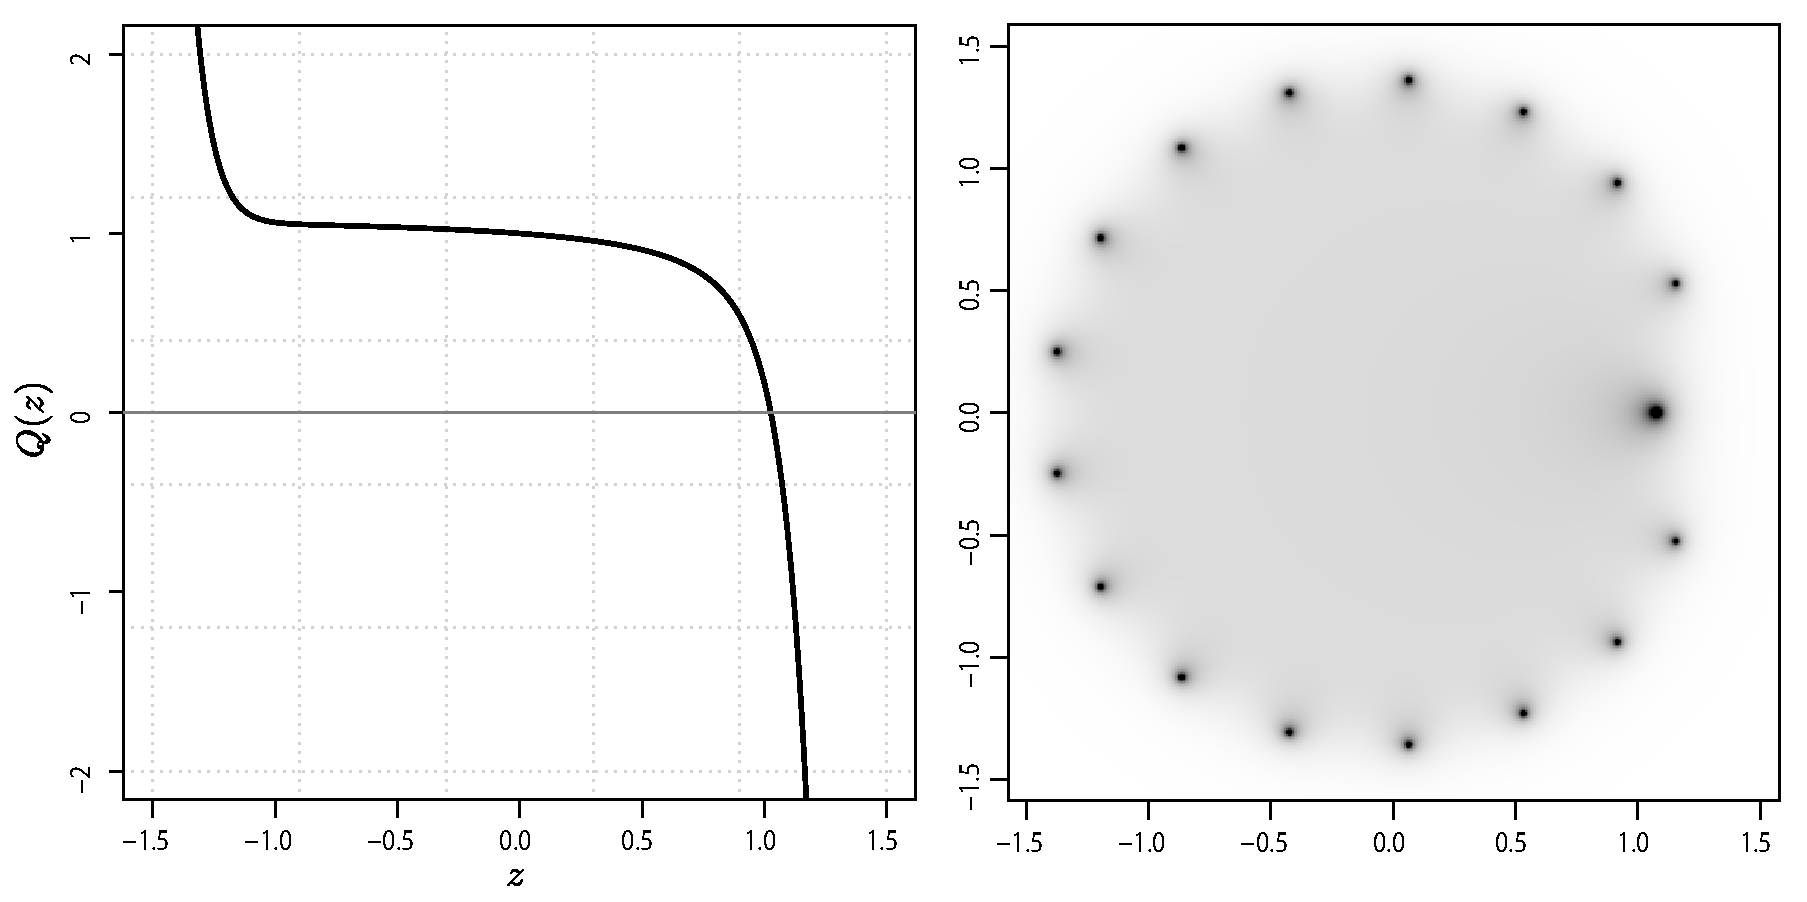
\includegraphics[scale=0.365]{singularityS.pdf}
\caption{\textbf{Singularities of $S$}. $Q(z)$ denotes the
denominator of $S(z)$ from expression (\ref{eq:Sp}). \textit{Left}: real
representation of $Q$. The bold line represents the value of $Q(z)$ for
$p=0.01$ and $d=17$. The root with smallest modulus appears in the
interval $(1, 1.5)$. \textit{Right}: complex representation of $Q$. Shown
is the complex plane around the origin. The darker the dot, the higher the
value of $1/Q(z)$ at the corresponding value of $z$. Sixteen singularities
of $S$ lie close to a circle. The remaining seventeenth is the one shown
on the left panel and it it is the dominant singularity because it lies
slightly closer to the origin.}
\label{fig:plotQ}
\end{figure}

The remaining singularities of $S(z)$ are complex and they seem to be
evenly spaced on the same circle, as can be seen on the right panel of
Figure~\ref{fig:plotQ}. This is only a visual impression. In fact the
singularities are not exactly on the same circle and their rotation angles
are not exactly regular.

%%%%%%%%%%%%% Minimal singularity of S %%%%%%%%%%%%%
\begin{proposition}
\label{th:roots}
$S$ has only one real positive singularity, which is the dominant
singularity.
\end{proposition}

\begin{proof}
Write $S(z) = P(z)/Q(z)$ and search the roots of $Q$. Let $x$ denote a
real number. Since $Q(1) = q^d > 0$ and $\lim_{x\rightarrow \infty} Q(x) =
-\infty$, $Q$ vanishes for a real number greater than $1$.
\end{proof}

We can now have all the tools to approximate the coefficients of $S(z)$
using proposition~\ref{th:ass} and thus obtain the approximate probability
that a read contains no seed.

\begin{proposition}
\label{th:p}
The probability that a read of of size $k$ is seedless is
asymptotically equivalent to

\begin{equation*}
\frac{C}{z_1^{k+2}},
\end{equation*}

\noindent
where $z_1$ is the only real positive root of the denominator of $S(z)$,
\textit{i.e.} the root of $1-pz(1+qz+\ldots+(qz)^{d-1})$ and

\begin{equation}
\label{eq:Cp}
C =\frac{(1-qz_1)^2}{p^2\left( 1 + d(qz_1)^{d+1} - (d+1)(qz_1)^d
\right)}.
\end{equation}

\end{proposition}

\begin{proof}
Apply proposition~\ref{th:ass} and proposition~\ref{th:roots} to $S(z)$
and also use the fact that $1+qz_1+\ldots+(qz_1)^{d-1} = 1/pz_1$.
\end{proof}

\begin{remark}
Since $z_1 > 1$, the probability decreases exponentially
as $k$ increases.
\end{remark}

We now illustrate proposition~\ref{th:p} with a concrete example
explaining how the calculations are done in practice.

\begin{example}
\label{ex:num}
Let us approximate the probability that a read of size $k=50$ is seedless
for $d=17$ and for a substitution rate $p=0.01$. To find the dominant
singularity of $S$, we need to solve $1-pz(1+qz+\ldots+(qz)^{16}) = 0$.
We rewrite the equation as $1-pz(1-(qz)^{17})/(1-qz) = 0$ and solve
it numerically with the Newton-Raphson method, yielding $z_1 \approx
1.026886$. Substituting this value in (\ref{eq:Cp}) yields $C \approx
1.433681$, so the probability that a read contains no seed is
approximately $1.433681 / 1.026886^{52} \approx 0.3608321$. For
comparison, performing 1,000,000 random simulations gives an estimate in
the range...
\end{example}

The demonstration of proposition~\ref{th:ass} shows that the analytic
combinatorics estimate converges exponentially as $k$ increases because
the dominant singularity has multiplicity $1$. The numerical estimates are
thus close to the exact values, as illustrated in example~\ref{ex:num}.
Figure~\ref{fig:simulp} shows this on more comprehensive example
with longer reads and higher probability of error $p$.

\begin{figure}[h]
\centering
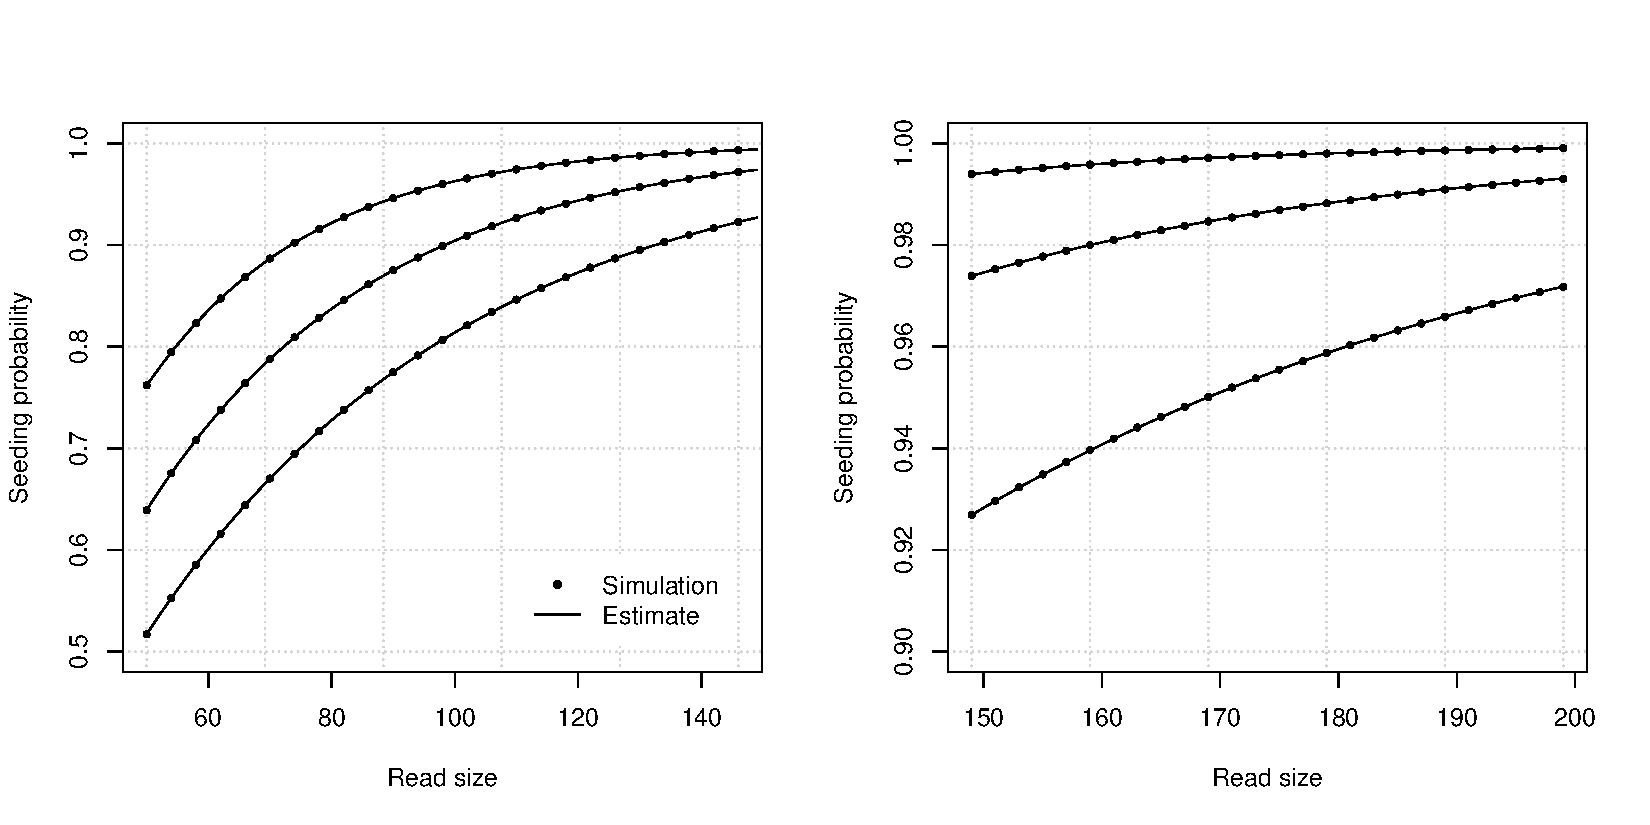
\includegraphics[scale=0.445]{simulp.pdf}
\caption{\textbf{Accuracy of the estimates}. The analytic combinatorics
estimates are compared to random simulations for $d=17$ and $p=0.08$,
$p=0.10$ or $p=0.12$. Shown on both panels are the probablities that a
read of given size contains a seed, either estimated by 10,000,000 random
simulations (dots), or by the method described above (lines). The
difference never exceeds 0.00028 on the examples shown here.}
\label{fig:simulp}
\end{figure}

Overall, the analytic combinatorics estimates are close to the exact
values. Figure~\ref{fig:simulp} also shows that relatively small changes
in the prboability of error have a large influence on the probability of
that the read contains a seed in the depicted range of read sizes.

\subsection{Substitutions and deletions}

The uniform substitution model does not describe all sequencing
technologies. For instance, long read technologies often have bursts of
insertions and deletions, with typical frequencies that differ from
substitutions. In order to model more complex behaviors, we need to
distinguish the different types of errors.

To not jump too fast into the problem, we will first focus on a fictional
case where errors can be deletions or susbtitutions. As in the case of
uniform substitutions, we assume that every nucleotide call is false with
a probability $p$ and true with a probability $1-p=q$. But here, we also
assume the ``space''  between consecutive nucleotides can contain a
deletion with probability $\delta$.

With this formalism, the weighted generating function of an error-only
interval of size $0$ is simply $\delta$. Whether the ``spaces'' between
the nucleotides of error-only intervals of size $k > 0$ contain deletions
or not is irrelevant. It also does not matter whether the interval starts
or ends with a deletion, so the weighted generating function of error-only
interval of size $k>1$ is $p^kz^k$. Finally, the $k-1$ ``spaces'' between
the nucleotides of an error-free interval of size $k$ must not contain any
deletion, so the weighted generating function of error-free intervals of
size $k>1$ is $(1-\delta)^{k-1}(pz)^k$. In summary $E(z) = \delta + pz +
(pz)^2 + \ldots = \delta + pz / (1-pz)$ and $F(z) = qz + (1-\delta)(qz)^2
+ (1-\delta)^2(qz)^3 + \ldots = qz / (1-(1-\delta)qz)$.

Substituting these values in equation (\ref{eq:R}), the weighted
generating function of reads appears as

\begin{equation*}
R(z) = \frac{\big(1+E(z)-E(0)\big)^2F(z)}{1-E(z)F(z)} + E(z)-E(0)+1 =
\frac{1}{1-z}.
\end{equation*}

The weighted generating function of the reads is the same as under the
constant substitution model, and the total weights are all equal to $1$.

The weighted generating function of error-free reads of size less than $d$
is $F_d(z) = qz + (1-\delta)(qz)^2 + \ldots + (1-\delta)^{d-2}(qz)^{d-1}$.
Substituting this value in equation (\ref{eq:S}), we obtain the
weighted generating function of seedless reads as

\begin{equation*}
\begin{split}
S(z) &= \frac{\big(1+E(z)-E(0)\big)^2F_d(z)}{1-E(z)F_d(z)} +
  E(z)-E(0)+1 \\
&= \frac{1+(1-\delta)\big(qz+(1-\delta)(qz)^2 + \ldots +
  (1-\delta)^{d-2}(qz)^{d-1}\big)}
  {1-pz - \big(pz(1-\delta) + \delta\big)\big(qz+(1-\delta)(qz)^2 +
  \ldots + (1-\delta)^{d-2}(qz)^{d-1}\big)}.
\end{split}
\end{equation*}

\begin{remark}
Setting $\delta = 0$ in the expression above, we obtain expression
(\ref{eq:Sp}), \textit{i.e.} the weighted generating function of seedless
reads when the only errors are substitutions.
\end{remark}

Applying proposition~\ref{th:ass} to this expression, we obtain the
following proposition.

\begin{proposition}
\label{th:pd}
The probability that a read of size $k$ is seedless is asymptotically
equivalent to

\begin{equation*}
\frac{C}{z_1^k},
\end{equation*}

\noindent
where $z_1$ is the only real positive root of the denominator of $S(z)$,
\textit{i.e.} the root of $1-pz - \big(pz(1-\delta) +
\delta\big)\big(qz+(1-\delta)(qz)^2 + \ldots +
(1-\delta)^{d-2}(qz)^{d-1}\big)$, and

\begin{equation}
\label{eq:Cpd}
\begin{split}
C &=
\frac{ \big(1-(1-\delta)(1-p)z\big)^2 }
{ \big((p+q\delta)z  -\gamma^*(1-\delta)^{d-1}(qz)^d \big)
\big(\delta+(1-\delta)pz\big) }, \\
\gamma^* &= d\delta -(1-\delta)\big((d-1)\delta-p((d-1)\delta+d+1)\big)z
- d(1-\delta)^2pqz^2.
\end{split}
\end{equation}
\end{proposition}

\begin{remark}
Notice that the power of $z_1$ differs between propositions~\ref{th:p} and
\ref{th:pd}. The reason is that the factors $z$ or $1/z$ have been moved
out of the constant $C$ in expressions (\ref{eq:Cp}) and (\ref{eq:Cpd}).
\end{remark}

\begin{example}
Let us approximate the probablity that a read of size $k = 100$ is
seedless for $d=17$ and for substitution and deletion rates $p = 0.05$ and
$\delta = 0.15$, respectively. In order to find the dominant singularity of
$S$, we need to solve the equation $1-pz - \big(pz(1-\delta) +
\delta\big)\big(qz+(1-\delta)(qz)^2 + \ldots +
(1-\delta)^{15}(qz)^{16}\big) = 0$. We rewrite it as $1-pz -
\big(pz(1-\delta)+\delta\big)(qz-(1-\delta)^{16}(qz)^{17}) /
(1-(1-\delta)qz) = 0$ and solve it numerically with the Newton-Raphson
method, yielding $z_1 \approx 1.006705$. Substituting this value in
(\ref{eq:Cpd}) yields $C \approx 1.088876$, so the probability that a read
contains no seed is approximately $1.088876 / 1.006705^{100} \approx
0.558141$. For comparison, performing 1,000,000 random simulations gives
an estimate in the range...
\end{example}

\begin{figure}[h]
\centering
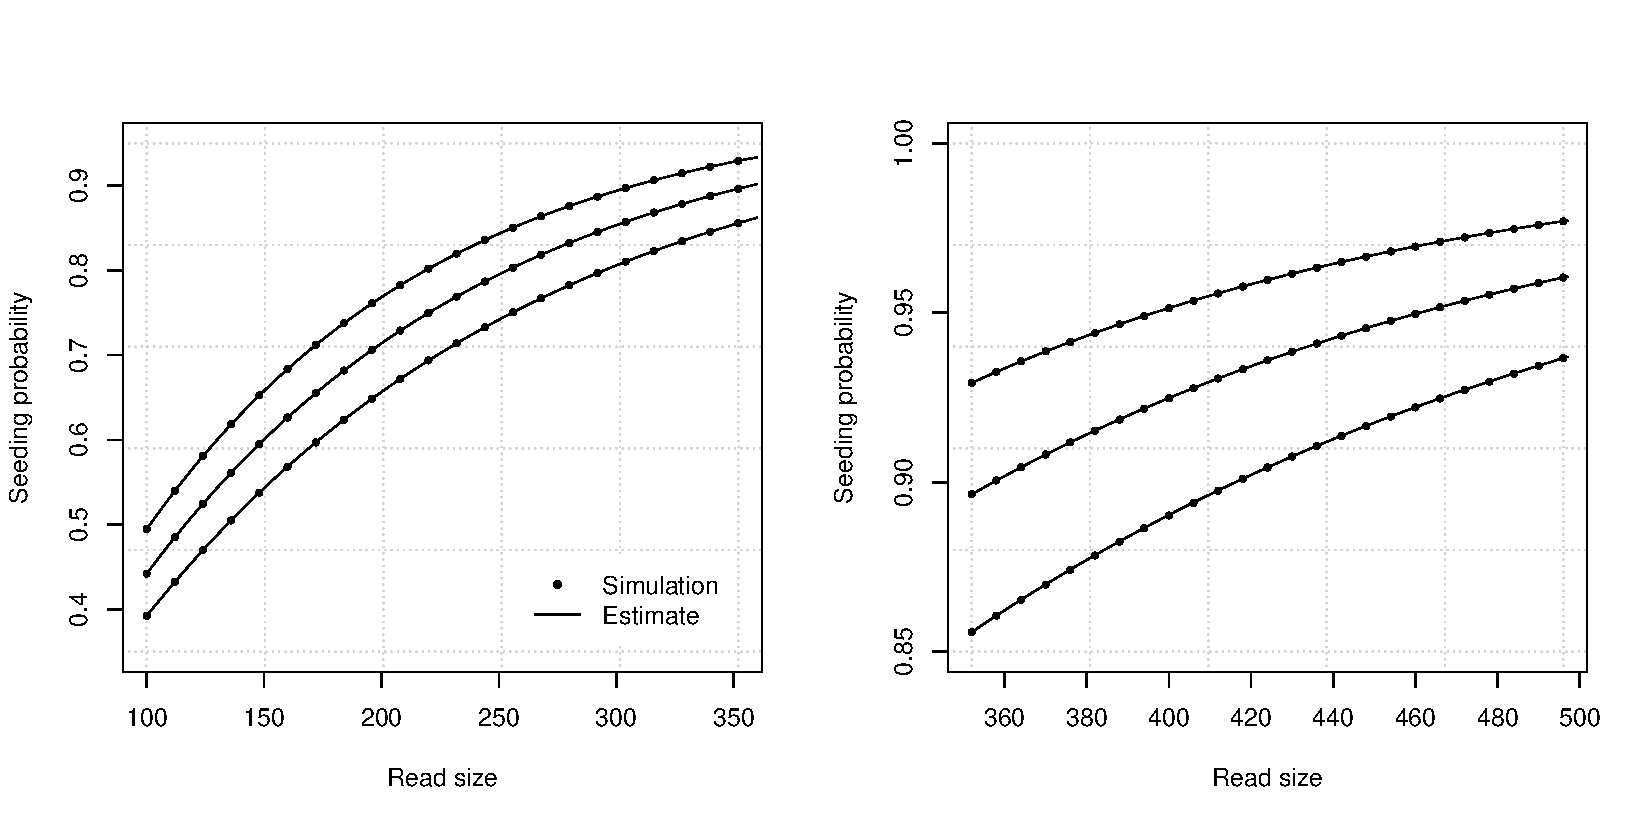
\includegraphics[scale=0.445]{simulpdel.pdf}
\caption{\textbf{Accuracy of the estimates}. The analytic combinatorics
estimates are compared to random simulations for $d=17$, $p=0.05$ and
$\delta=0.14$ or $\delta=0.15$ or $\delta=0.16$. Shown on both panels are
the probablities that a read of given size contains a seed, either
estimated by 10,000,000 random simulations (dots), or by the method
described above (lines). The difference never exceeds 0.0004 on the
examples shown here.}
\label{fig:simulpdel}
\end{figure}

\subsection{Substitutions, deletions and insertions}

\begin{figure}[h]
\centering
\includegraphics[scale=0.83]{sketch_errors.pdf}
\caption{\textbf{Complex error models}.
Text.
}
\label{fig:sketcherr}
\end{figure}

\section{Inexact seeding}

We now consider a more challenging problem. The ongoing development of
algorithms and data structures allows us to use...

Here we assume the constant substitution rate model.

\begin{definition}
\label{def:seed}
An inexact $d$-seed is an interval of size at least $d$ that contains at
most a bustitution and no other error. An exact $d$-seed is an inexact
$d$-seed, but the converse is not true.
\end{definition}

In other words, an inexact seed is either an error-free interval or the
concatenation of two error-free intervals and a substitution, each with
total size at least $d$. In this context, a ``seedless'' read will
designate a read that does not contain any inexact seed.

As in the case of exact seeding, we will give a construction of seedless
reads, find the corresponding weighted generating function and extract the
asymptotic behavior of the coefficients. The main difference with the
previous case is that seedless reads are not simple sequences of
intervals. The error-free intervals on either side of the substitution are
linked by the constraint that their total size cannot be larger than $d-2$
(the read must not contain a inexact $d$-seed, and the substitution has
size $1$).

Following remark~\ref{rem:alt}, it is more convenient to segment seedless
reads in a slightly different way.

The easiest way to encode this dependence is to design a transition matrix
$M$, such that the entry at position $(i,j)$ is the weighted generating
function of a substitution and an error-free intervals of size $j$ on the
right-hand-side of an error-free interval of size $i+1$. For instance, the
term at position $(1,1)$ is always $qz$ (provided $d \geq 3$). This
corresponds to appending an error-free interval of size $1$ to an
error-free interval and a substitution.

The general format of the matrix is

\begin{equation}
M = pz\left[
\begin{matrix}
1 & qz  & (qz)^2 & (qz)^3 & \ldots & (qz)^{d-3} & (qz)^{d-2} \\
1 & qz  & (qz)^2 & (qz)^3 & \ldots & (qz)^{d-3} & 0          \\
1 & qz  & (qz)^2 & (qz)^3 & \ldots & 0          & 0          \\
\vdots & \vdots & \vdots & \vdots & \ddots & \vdots & \vdots \\
1 & qz  & (qz)^2 & 0      & \ldots & 0          & 0          \\
1 & qz  & 0      & 0      & \ldots & 0          & 0          \\
1 & 0   & 0      & 0      & \ldots & 0          & 0
\end{matrix}
\right]
\end{equation}

The term at position $(i,j)$ in the matrix $M^n$ is the generating
function of reads with $n+1$ error-free intervals (possibly empty), whose
first interval has size $i-1$ and whose last interval has size $j-1$.

The vector $pz(1, qz, (qz)^2, \ldots, (qz)^{d-2})$.



%---------------------------------------------------------------
%---------------------------------------------------------------

\bibliography{pubmed,extra}
\bibliographystyle{plain}

%----------------------------------------------------------------

\end{document}

%gs -dNoOutputFonts -sDEVICE=pdfwrite -o out.pdf latex.pdf 
